\section{Pretraining Details}

\subsection{Pretraining Datasets}
\label{app:audio_text_data_details}
For image-text pairs, we use LAION-2B~\cite{laion5b}, a dataset obtained by web crawling that may contain some noisy pairs. 
To improve the data quality, we apply several pre-processing steps, including removing images with an aspect ratio greater than 3.5, removing images with the shortest side less than 128, and removing images with a CLIP score less than 0.3. We also remove texts containing non-English or emoji characters, as well as texts with lengths less than 3 or greater than 512. 
After these steps, we retain about 1.5 billion image-text pairs.

For audio-text pairs, we mainly use the environmental sound datasets processed by \cite{laion_clap}. Specifically, for some datasets that only contain tags, \cite{laion_clap} uses a pretrained language model T5~\cite{T5} to rewrite these tags into captions.
We also perform simple cleaning on the data, which involves removing samples with text lengths less than 3 or greater than 512, as well as texts containing non-English or emoji characters. 
Ultimately, we obtain about 2.4 million audio-text pairs, with a total duration of around 8,000 hours.
Table~\ref{tb:audio_dataset} presents the environmental sound datasets utilized by \onepeace.

% \begin{table*}[h]
% \centering
% \caption{Statistics on the environmental sound datasets. All datasets are publicly available.}
% % For language data, 140GB represents the storage space of the plain texts.}
% \vskip 0.15in
% \begin{adjustbox}{max width=1.\textwidth}
% \begin{tabular}{@{\extracolsep{\fill}}cccc}
% \toprule
%   Dataset
%   & Number of Samples
%   & Duration
%   & T5 Augmentation
%   \\
% \midrule
%   Epidemic Sound & 75618 & 220.40 hrs & Yes
%   \\ 
%   AudioCaps~\cite{audiocaps} & 49494 & 135.56 hrs & No
%   \\
%   AudioSet~\cite{audioset} & 1910918 & 5263.23 hrs & Yes
%   \\
%   AudioStock & 9552 & 40.31 hrs & No
%   \\
%   Clotho~\cite{clotho} & 3839 & 23.99 hrs & No
%   \\ 
%   Freesound~\cite{freesound} & 363618 & 2162.10 hrs & No
%   \\
%   MACS & 3537 & 9.85 hrs & No
%   \\ 
%   Sounddescs~\cite{sounddescs} & 10677 & 331.67 hrs & No
%   \\
%   Wavtext5K~\cite{wavtext5k} & 2248 & 17.23 hrs & No
%   \\
% \bottomrule
% \end{tabular}
% \end{adjustbox}
% \label{tb:audio_dataset}
% \end{table*}


\begin{table*}[h]
\centering
\normaltablestyle{8pt}{1.2}
\begin{tabular}{l|ccc}
  Dataset
  & Number of Samples
  & Duration
  & T5 Augmentation
  \\
  \shline
  Epidemic Sound & 75618 & 220.40 hrs & Yes
  \\ 
  AudioCaps~\cite{audiocaps} & 49494 & 135.56 hrs & No
  \\
  AudioSet~\cite{audioset} & 1910918 & 5263.23 hrs & Yes
  \\
  AudioStock & 9552 & 40.31 hrs & No
  \\
  Clotho~\cite{clotho} & 3839 & 23.99 hrs & No
  \\ 
  FreeSound~\cite{freesound} & 363618 & 2162.10 hrs & No
  \\
  MACS & 3537 & 9.85 hrs & No
  \\ 
  SoundDescs~\cite{sounddescs} & 10677 & 331.67 hrs & No
  \\
  WavText5K~\cite{wavtext5k} & 2248 & 17.23 hrs & No
  \\
\end{tabular}
\caption{\textbf{Statistics on the environmental sound datasets.} All datasets are publicly available.}
\label{tb:audio_dataset}
\end{table*}

\subsection{Pretraining Settings}
\label{app:pretraining_hyperparameters}
% We divide the pretraining of \onepeace into two stages: vision-language pretraining and audio-language pretraining.
% During the vision-language pretraining stage, the model trains on image-text pairs and only updates parameters that are relevant to vision and language.
% For each image-text pair, we not only utilize them to calculate $\mathcal{L}_{CL-VL}$ and $\mathcal{L}_{MCL-VL}$, but also separately using the image and text to calculate $\mathcal{L}_{MCL-V}$ and $\mathcal{L}_{MCL-L}$ respectively.
% The loss function at this stage is shown below:

% \begin{equation}
% \mathcal{L}_{VL} = \mathcal{L}_{CL-VL} + 1.0*\mathcal{L}_{MCL-V} + 0.5*\mathcal{L}_{MCL-L} + 1.0*\mathcal{L}_{MCL-VL}
% \end{equation}

% During the audio-language pretraining stage, the model trains on audio-text pairs, and we only update A-Adapter, A-FFNs, and other audio-related parameters. 
% The remaining parameters including self-attention layers are totally frozen.
% Despite not training on image-audio pairs, the semantic space between vision and audio is still aligned by using language as the anchor.
% The loss function at the audio-language pretraining stage is shown below:

% \begin{equation}
% \mathcal{L}_{AL} = \mathcal{L}_{CL-AL} + 1.0*\mathcal{L}_{MCL-A} + 1.0*\mathcal{L}_{MCL-AL}
% \end{equation}


As mentioned in Sec~\ref{sec:two_stage_pretraining}, the pretraining of \onepeace is divided into two stages: vision-language pretraining and audio-language pretraining.

For vision-language pretraining, we pretrain \onepeace for 200K steps with a batch size of 32768. We use the AdamW~\cite{adamw} optimizer with $(\beta_1,\beta_2)=(0.9, 0.98)$ and $\epsilon=1e\text{-}8$. The peak learning rate is set to $5e-4$, with a linear warmup of $3000$ steps and a cosine decay scheduler. The image resolution is set to $256\times256$. The maximum text sequence length is set to 70. For regulation, we use weight decay with $0.05$ and disable dropout. We employ drop path~\cite{drop-path} with a $0.4$ rate.

For audio-language pretraining, we keep the model parameters related to vision and language (e.g., self-attention layers) frozen and only update the parameters that pertain to audio, such as A-Adapter and A-FFN.
In this stage, we pretrain \onepeace for $10$ epochs with a batch size of $3072$. The peak learning rate is set to $2e-4$, with a linear warmup of $1$ epoch and cosine decay scheduler. The maximum audio duration is set to $15$s. For audio with a duration of less than $1$s, we first repeat the input and then truncate it to $1$s.
Other hyper-parameters remain the same as vision-language pretraining.

% The model weights of \onepeace are randomly initialized at the beginning, except for the feature extractor of audio-adapter, for which we use the weights of WavLM~\cite{wavlm} for initialization. We find that a randomly initialized feature extractor can lead to overfitting, whereas incorporating the weights from WavLM significantly mitigated this problem and improve the performance.


% We mainly use the environmental sound datasets processed by \cite{laion_clap}. Specifically, for some datasets that only contain tags, \cite{laion_clap} uses a pretrained language model T5~\cite{T5} to rewrite these tags into captions.
% The experimental results in~\cite{laion_clap} show that these augmented captions can improve the performance of the model in various downstream speech tasks. 
% Table~\ref{tb:audio_dataset} presents the environmental sound datasets utilized by \onepeace.

\section{Details of Downstream Tasks}
\label{app:downstream_tasks}
% Here we describe the implementation details of different downstream tasks, including vision-language tasks, vision tasks, and audio tasks.

\subsection{Vision Tasks}
\label{app:vision_details}
Here we describe the implementation details of different vision tasks, including image classification~\cite{inet1k}, semantic segmentation~\cite{Zhou2016SemanticUO}, object detection~\cite{mscoco}, and video action recognition~\cite{k400}.
All detailed hyperparameters are listed in Table~\ref{tb:v_task_config}.

\paragraph{Image Classification}
We provide the fine-tuning results on ImageNet-1k~\cite{inet1k}. Following recent studies in self-supervised learning for computer vision, we use global pooling of all image tokens excluding the class token, and append a LayerNorm with a linear layer for classification. To further unleash the potential of \onepeace, we perform intermediate fine-tuning on ImageNet-21k~\cite{imagenet}. We set the label smoothing as 0.3 and do not use random erasing, mixup, and cutmix data augmentations. For fine-tuning on ImageNet-1k, we use exponential moving average (EMA) for model parameters and set the EMA decay rate as 0.9998. For intermediate fine-tuning on ImageNet-21k, we do not use EMA. We also use Zero Redundancy Optimizer~\cite{zero} and set the stage as 1.

\paragraph{Semantic Segmentation}
We provide the fine-tuning results on ADE20k~\cite{Zhou2016SemanticUO}. We use Mask2Former~\cite{mask2former} as the segmentation head. We first intermediate fine-tune segmentation head on coco-stuff~\cite{cocostuff} dataset for 80k steps. The learning rate is set as 2e-5 and the rest hyperparameters are the same as ADE20K shown in Table~\ref{tb:v_task_config}. Then we fine-tune the model on ADE20K. Both experiments use the cosine learning rate decay scheduler.

\paragraph{Object Detection}
We provide the fine-tuning results on COCO~\cite{mscoco} with ViTDet~\cite{vitdet}. We use large-scale jitter~\cite{lsj} data augmentation and fine-tune for 50 epochs. We use the linear learning rate decay scheduler and decay the learning rate at 44 and 48 epochs respectively.

\paragraph{Video Action Recognition}
To perform video action recognition, following AIM~\cite{aim}, we freeze the parameters of the pre-trained model and add spatial and temporal MLP adapters in each transformer layer. We conduct experiments on Kinetics 400~\cite{k400} dataset. Due to the invalid video links, there are many different versions of the K400 dataset and we use the version released on AcademicTorrents. We use the cosine learning decay scheduler and set the backbone learning rate multiplier of 0.1.

\begin{table*}[t]
\normaltablestyle{8pt}{1.2}
\begin{tabular}{y{96}|ccccc}
Config & ImageNet-21k & ImageNet-1k & ADE20K & COCO & Kinetics 400\\
\shline
Optimizer & \multicolumn{5}{c}{AdamW} \\
Optimizer momentum & \multicolumn{5}{c}{$\beta_1, \beta_2{=}0.9, 0.999$} \\
Numerical precision & \multicolumn{5}{c}{$\mathtt{fp16}$} \\
Peak learning rate & 1e-4 & 5e-5 & 1.5e-5 & 1e-4 & 3e-4 \\
Layer-wise lr decay & 0.85 & 0.9 & 0.95 & 0.9 & - \\
Weight decay & 0.05 & 0.05 & 0.05 & 0.1 & 0.05 \\
Batch size & 5120 & 1024 & 16 & 64 & 64 \\
Warmup ratio & 0.375 & 0.2 & 0.0375 & 0.003 & 0.1 \\
Training epochs & 40 & 15 & 30 & 50 & 30 \\
%augmentation & RandAug (9, 0.5) \\
Drop path & 0.4 & 0.4 & 0.5 & 0.6 & 0.4 \\
Image resolution & 256$^2$ & 512$^2$ & 896$^2$ & 1280$^2$ & 256$^2$ \\
\end{tabular}
\caption{\textbf{Fine-tuning setting for vision tasks.}}
\label{tb:v_task_config}
\end{table*}

\subsection{Audio-(language) Tasks}
\label{app:audio_details}

We describe the implementation details of audio-text retrieval, audio classification, and audio question answering here. All detailed hyperparameters are listed in Table~\ref{tb:audio_config}.

\begin{table*}[h]
\normaltablestyle{8pt}{1.1}
\begin{tabular}{y{96}|cccc}
Config & AudioCaps \& Clotho & FSD50K & VGGSound & AQA \\
\shline
Optimizer & \multicolumn{4}{c}{AdamW} \\
Optimizer momentum & \multicolumn{4}{c}{$\beta_1, \beta_2{=}0.9, 0.999$} \\
Weight decay & \multicolumn{4}{c}{0.05} \\
Gradient clip & \multicolumn{4}{c}{0.0} \\
Warmup ratio & \multicolumn{4}{c}{0.1} \\
Learning rate schedule & \multicolumn{4}{c}{cosine decay} \\
Numerical precision & \multicolumn{4}{c}{$\mathtt{bf16}$} \\
Peak learning rate & 1.5e-4 & 1e-4 & 8e-5 & 7e-5 \\
Layer-wise lr decay & 0.95 & 0.9 & 0.95 & 0.9  \\
Batch size & 384 & 128 & 512 & 128 \\
Training epochs & 10 & 10 & 10 & 10 \\
Drop path & 0.9 & 0.5 & 0.6 & 0.5 \\
Max duration & 20s & 15s & 15s & 15s \\
\end{tabular}
\caption{\textbf{Fine-tuning setting for audio(-language) tasks.}}
\label{tb:audio_config}
\end{table*}

\paragraph{Audio-Text Retrieval}
We evaluate \onepeace on AudioCaps~\cite{audiocaps} and Clotho~\cite{clotho} datasets.
To get better results, we merge the training set of AudioCaps~\cite{audiocaps}, Clotho~\cite{clotho}, and MACS as the fine-tuning dataset.
Similar to image-text retrieval, we use A-Branch and L-Branch to extract the features of audio clips and texts respectively, and then calculate the cosine similarity between these features.
The recall@k is employed as the evaluation metric.

\paragraph{Audio Classification}
We conduct experiments on three datasets: ESC-50~\cite{esc50}, FSD50K~\cite{fsd50k}, and VGGSound~\cite{vggsound}. 
ESC-50 is an environmental sound dataset that contains $2000$ environmental audio recordings and $50$ labels. 
We directly use the pretrained \onepeace model to perform zero-shot audio classification on ESC-50. Specifically, we use A-Branch to extract audio embeddings from the audio clips and use L-Branch to extract text embeddings from the label names. Then we determine the labels of the audio clips by calculating the similarity between the embeddings.
For FSD50K and VGGSound, we input the original audio into the A-Branch and utilize multi-head attention pooling (MAP) to aggregate the features. 
FSD50K is a multi-label sound event dataset, for which we use BCELoss as the loss function and report the mean average precision on the test set.
VGGSound is an audio-visual dataset, where each sample includes a video with audio.
We extract the audio clips from the videos and excluded the visual information, using cross entropy as the loss function and reporting accuracy on the test set.

\paragraph{Audio Question Answering}
We conduct experiments on the AVQA dataset~\cite{avqa}. 
Each sample in this dataset consists of a video, a question, and four candidate answers. 
To perform the audio question answering task, we extract audio clips from the videos and excluded the visual information. 
During training, we concatenate each answer with the audio and question, and extracted the features through AL-Branch. 
We then minimize the pairwise hinge loss between the positive features and negative features.


\subsection{Vision-language tasks}
\label{app:vision_language_details}
Here we describe the implementation details of different vision-language tasks, including image-text retrieval~\cite{flickr,mscoco}, visual grounding~\cite{refcoco,refcocog}, visual question answering~\cite{vqa}, and visual reasoning~\cite{nlvr2}.
All detailed hyperparameters are listed in Table~\ref{tb:vision_language_config}.

\begin{table*}[h]
\normaltablestyle{8pt}{1.2}
\begin{tabular}{y{96}|cccccc}
Config & MSCOCO & Flickr30K & RefCOCO/$+$/g & VQA & NLVR2 \\
\shline
Optimizer & \multicolumn{5}{c}{AdamW} \\
Optimizer momentum & \multicolumn{5}{c}{$\beta_1, \beta_2{=}0.9, 0.999$} \\
Weight decay & \multicolumn{5}{c}{0.05} \\
Gradient clip & \multicolumn{5}{c}{0.0} \\
Warmup ratio & \multicolumn{5}{c}{0.1} \\
Learning rate schedule & \multicolumn{5}{c}{cosine decay} \\
Numerical precision & \multicolumn{5}{c}{$\mathtt{bf16}$} \\
Peak learning rate & 8e-5 & 7e-5 & 1.5e-4 & 3e-4 & 1e-4 \\
Layer-wise lr decay & 0.9 & 0.9 & 0.9 & 0.85 & 0.9 \\
Batch size & 3072 & 3072 & 256 & 512 & 128 \\
Training epochs & 15 & 20 & 30 & 10 & 25 \\
Drop path & 0.5 & 0.4 & 0.4 & 0.5 & 0.4 \\
Image resolution & 432 & 432 & 384 & 768 & 256 \\
\end{tabular}
\caption{\textbf{Fine-tuning setting for vision-language tasks.}}
\label{tb:vision_language_config}
\end{table*}

\paragraph{Image-Text Retrieval}
We evaluate \onepeace on MSCOCO~\cite{mscoco} and Flickr30K~\cite{flickr} datasets, and report the results on the widely used Karpathy test split~\cite{karpathy}.
We use V-Branch and L-Branch to extract the features of images and texts respectively, and then calculate the cosine similarity between these features.
The recall@k is employed as the evaluation metric.

\paragraph{Visual Grounding}
This task requires the model to locate an image region based on a text description.
We conduct experiments on RefCOCO, RefCOCO+, and RefCOCOg datasets~\cite{refcoco,refcocog}.
The image and text are fed to the VL-Branch simultaneously, then we use multi-head attention pooling (MAP)~\cite{set_transformer} to aggregate the features from all image patches.
The pooled output is used to predict the continuous corner coordinates of the bounding box $\left(x_1,y_1,x_2,y_2 \right)$, where $x_1$ and $y_1$ denotes the normalized top left coordinates, $x_2$ and $y_2$ denotes the normalized bottom right coordinates.
We report the standard metric Acc@0.5 on the validation and test sets.

\paragraph{Visual Question Answering}
This task requires the model to answer the question based on an image. We perform experiments on the VQAv2 dataset~\cite{vqav2}.
Following previous works~\cite{ofa,albef,blip,x-vlm}, we use the training and validation set of VQAv2 for training, including additional question-answer pairs from Visual Genome~\cite{vg}.
The image and question are fed to the VL-Branch simultaneously, then we use MAP to aggregate the features from all text tokens.
The pooled output is fed into a classifier to predict the answer from the 3,129 most frequent answers.
We report the final score on the test-dev and test-std sets.

% \paragraph{Visual Entailment}
% Visual entailment requires the model to predict the relationship between an image and a text hypothesis, i.e., entailment, neutral, or contradiction.
% We conduct experiments on the SNLI-VE dataset~\cite{snli-ve}.
% Similar to VQA, the given image and text hypothesis are fed to the VL-Branch.
% The final pooled output is fed into a classifier to predict the label.

\paragraph{Visual Reasoning}
Given a text and a pair of images, this task requires the model to distinguish whether the text truly describes the images. We conduct experiments on the NLVR2 dataset~\cite{nlvr2}.
Following the common practice, We treat each sample as two image-text pairs, each containing a text and one image. Then we input these pairs into VL-branch respectively.
The final pooled outputs are concatenated together and fed to a classifier to predict the label. 
We report accuracy on the dev and test-P sets.

% \subsection{Vision Tasks}
% \label{app:vision_details}
% Here we describe the implementation details of different vision tasks, including image classification~\cite{inet1k}, semantic segmentation~\cite{Zhou2016SemanticUO}, object detection~\cite{mscoco}, and video action recognition~\cite{k400}.
% All detailed hyperparameters are listed in Table~\ref{tb:v_task_config}.

% \paragraph{Image Classification}
% We provide the fine-tuning results on ImageNet-1k~\cite{inet1k}. Following recent studies in self-supervised learning for computer vision, we use global pooling of all image tokens excluding the class token, and append a LayerNorm with a linear layer for classification. To further unleash the potential of \onepeace, we optionally intermediate fine-tune on ImageNet-21k~\cite{imagenet}. We set the label smoothing as 0.3 and do not use random erasing, mixup, and cutmix data augmentations. For fine-tuning on ImageNet-1k, we use ema for model parameters and set the ema decay rate as 0.9998. For intermediate fine-tuning on ImageNet-21k, we do not use ema. We also use Zero Redundancy Optimizer~\cite{zero} and set the stage as 1.

% \paragraph{Semantic Segmentation}
% We provide the fine-tuning results on ADE20k~\cite{Zhou2016SemanticUO}. We use Mask2Former~\cite{mask2former} as the segmentation head. We first intermediate fine-tune segmentation head on coco-stuff~\cite{cocostuff} dataset for 80k steps. The learning rate is set as 2e-5 and the rest hyperparameters are the same as ADE20K shown in Table~\ref{app:vision_details}. Then we fine-tune the model on ADE20K. Both experiments use the cosine learning rate decay scheduler.

% \paragraph{Object Detection}
% We provide the fine-tuning results on COCO~\cite{mscoco} with ViTDet~\cite{vitdet}. We use large-scale jitter~\cite{lsj} data augmentation and fine-tune for 50 epochs. We use the linear learning rate decay scheduler and decay the learning rate at 44 and 48 epochs respectively.

% \paragraph{Video Action Recognition}
% To perform video action recognition, following AIM~\cite{aim}, we freeze the parameters of the pre-trained model and add spatial and temporal MLP adapters in each transformer layer. We conduct experiments on Kinetics 400~\cite{k400} dataset. Due to the invalid video links, there are many different versions of the K400 dataset and we use the version released on AcademicTorrents. We use the cosine learning decay scheduler and set the backbone learning rate multiplier of 0.1.

% \begin{table*}[t]
% \normaltablestyle{8pt}{1.2}
% \begin{tabular}{y{96}|ccccc}
% Config & ImageNet-1k & ImageNet-21k & ADE20K & COCO & Kinetics 400\\
% \shline
% Optimizer & \multicolumn{5}{c}{AdamW} \\
% Optimizer momentum & \multicolumn{5}{c}{$\beta_1, \beta_2{=}0.9, 0.999$} \\
% Numerical precision & \multicolumn{5}{c}{$\mathtt{fp16}$} \\
% Peak learning rate & 5e-5 & 1e-4 & 1.5e-5 & 1e-4 & 3e-4 \\
% Layer-wise lr decay & 0.9 & 0.85 & 0.95 & 0.9 & - \\
% Weight decay & 0.05 & 0.05 & 0.05 & 0.1 & 0.05 \\
% Batch size & 1024 & 5120 & 16 & 64 & 64 \\
% Warmup ratio & 0.2 & 0.375 & 0.0375 & 0.003 & 0.1 \\
% Training epochs & 15 & 40 & 30 & 50 & 30 \\
% %augmentation & RandAug (9, 0.5) \\
% Drop path & 0.4 & 0.4 & 0.5 & 0.6 & 0.4 \\
% Image resolution & 518$^2$ & 256$^2$ & 896$^2$ & 1280$^2$ & 256$^2$ \\
% \end{tabular}
% \caption{\textbf{Fine-tuning setting} for vision tasks.}
% \label{tb:v_task_config}
% \end{table*}

% \subsection{Audio-(language) Tasks}
% \label{app:audio_details}

% We describe the implementation details of audio-text retrieval and audio classification tasks here. All detailed hyperparameters are listed in Table~\ref{tb:audio_config}.

% \begin{table*}[h]
% \normaltablestyle{8pt}{1.2}
% \begin{tabular}{y{96}|ccc}
% Config & AudioCaps \& Clotho & FSD50K & VGGSound \\
% \shline
% Optimizer & \multicolumn{3}{c}{AdamW} \\
% Optimizer momentum & \multicolumn{3}{c}{$\beta_1, \beta_2{=}0.9, 0.999$} \\
% Weight decay & \multicolumn{3}{c}{0.05} \\
% Gradient clip & \multicolumn{3}{c}{0.0} \\
% Warmup ratio & \multicolumn{3}{c}{0.1} \\
% Learning rate schedule & \multicolumn{3}{c}{cosine decay} \\
% Numerical precision & \multicolumn{3}{c}{$\mathtt{bf16}$} \\
% Peak learning rate & 1.5e-4 & 1e-4 & 8e-5 \\
% Layer-wise lr decay & 0.95 & 0.9 & 0.95  \\
% Batch size & 384 & 128 & 512 \\
% Training epochs & 10 & 10 & 10 \\
% Drop path & 0.9 & 0.5 & 0.6 \\
% Max duration & 20s & 15s & 15s \\
% \end{tabular}
% \caption{\textbf{Fine-tuning setting} for audio(-language) tasks}
% \label{tb:audio_config}
% \end{table*}

% \paragraph{Audio-Text Retrieval}
% We evaluate \onepeace on AudioCaps~\cite{audiocaps} and Clotho~\cite{clotho} datasets.
% To get better results, we merge the training set of AudioCaps~\cite{audiocaps}, Clotho~\cite{clotho}, and MACS as the fine-tuning dataset.
% Similar to image-text retrieval, we use A-Branch and L-Branch to extract the features of audio clips and texts respectively, and then calculate the cosine similarity between these features.
% The recall@k is employed as the evaluation metric.

% \paragraph{Audio Classification}
% We conduct experiments on three datasets: ESC-50~\cite{esc50}, FSD50K~\cite{fsd50k}, and VGGSound~\cite{vggsound}. 
% ESC-50 is an environmental sound dataset that contains $2000$ environmental audio recordings and $50$ labels. 
% We directly use the pretrained \onepeace model to perform zero-shot audio classification on ESC-50. Specifically, we use the A-Branch to extract audio embeddings from the audio clips and use L-Branch to extract text embeddings from the label names. Then we determine the labels of the audio clips by calculating the similarity between the embeddings.
% For FSD50K and VGGSound, we input the original audio into the A-Branch and utilize multi-head attention pooling (MAP) to aggregate the features. 
% FSD50K is a multi-label sound event dataset, for which we use BCELoss as the loss function and report the mean average precision on the test set.
% VGGSound is an audio-visual dataset, where each sample includes a video with audio.
% We extract the audio clips from the videos and excluded the visual information, using cross entropy as the loss function and reporting accuracy on the test set.

\section{Effects of Pretrained Audio Feature Extractor}
\label{app:audio_feature_extractor}

We conduct a systematic analysis of the impact of the pretrained audio feature extractor.
We find that although the parameters of the feature extractor are only $4.6$M, accounting for only about $1\%$ of the total parameters, it has a significant impact on the model performance. 
As shown in Table~\ref{tb:audio_ablation}, the feature extractor with random initialization only achieves $85.3$ accuracy on the ESC-50 dataset, while using pretrained feature extractors results in better performance. 
Notably, using the WavLM feature extractor can lead to the largest improvement (+6.2).
 We attribute this to the fact that WavLM is trained on a more diverse audio dataset compared to Hubert and Wav2Vec 2.0, making its feature extractor more suitable for environmental sound tasks.

 \begin{table*}[h]
\centering
\normaltablestyle{6pt}{1.3}
\begin{tabular}{c|cccc}
  Feature Extractor & Random Init. & Init. with Hubert~\cite{hubert} & Init. with Wav2Vec 2.0~\cite{wav2vec2} & Init. with WavLM~\cite{wavlm}
  \\
  \shline
  ESC-50 Acc. & 85.8 &89.6 (+3.8)  & 90.0 (+4.2) & 91.8 (+6.0)
  \\
\end{tabular}
\caption{\textbf{Ablation studies of pretrained audio feature extractors.} We report zero-shot accuracy on the ESC-50 dataset.}
\label{tb:audio_ablation}
\end{table*}


\section{Evaluate \onepeace on \textit{One Piece}}
\label{app:one_piece}
We further test the visual grounding ability of \onepeace by using a more complex anime picture, \textit{One Piece}. 
The model is fine-tuned on the RefCOCOg dataset.
As shown in Figure~\ref{fig:onepiece_grounding_visual}, we ask \onepeace to locate the characters based on their names. Although \onepeace hasn't seen any anime pictures in the RefCOCOg dataset, it still achieves a recognition accuracy of 56.6\%.

\label{app:visual_grounding_onepiece}
\begin{figure*}[t]
    \centering
    
\includegraphics[width=\linewidth]{pic/onepiece_grounding_visual.pdf}
    \caption{Visualization of \onepeace locating different characters of \textit{One Piece}. Given the names of 9 members of the Straw Hat Pirates, \onepeace correctly located 5 of them from the picture.}
    \label{fig:onepiece_grounding_visual}
\end{figure*}

\section{More Examples of Emergent Zero-shot Retrieval}
\label{app:emergent_zero_shot}

In this section, we provide more examples to demonstrate the emergent zero-shot abilities of \onepeace, including audio-to-image, audio+image-to-image, and audio+text-to-image retrieval.
The audios are selected from ESC-50~\cite{esc50}, and the images are retrieve from ImageNet-1K~\cite{imagenet} and MSCOCO~\cite{mscoco}.
By reading this section, we hope that readers can better perceive \onepeace.

\begin{figure*}[t]
    \centering
    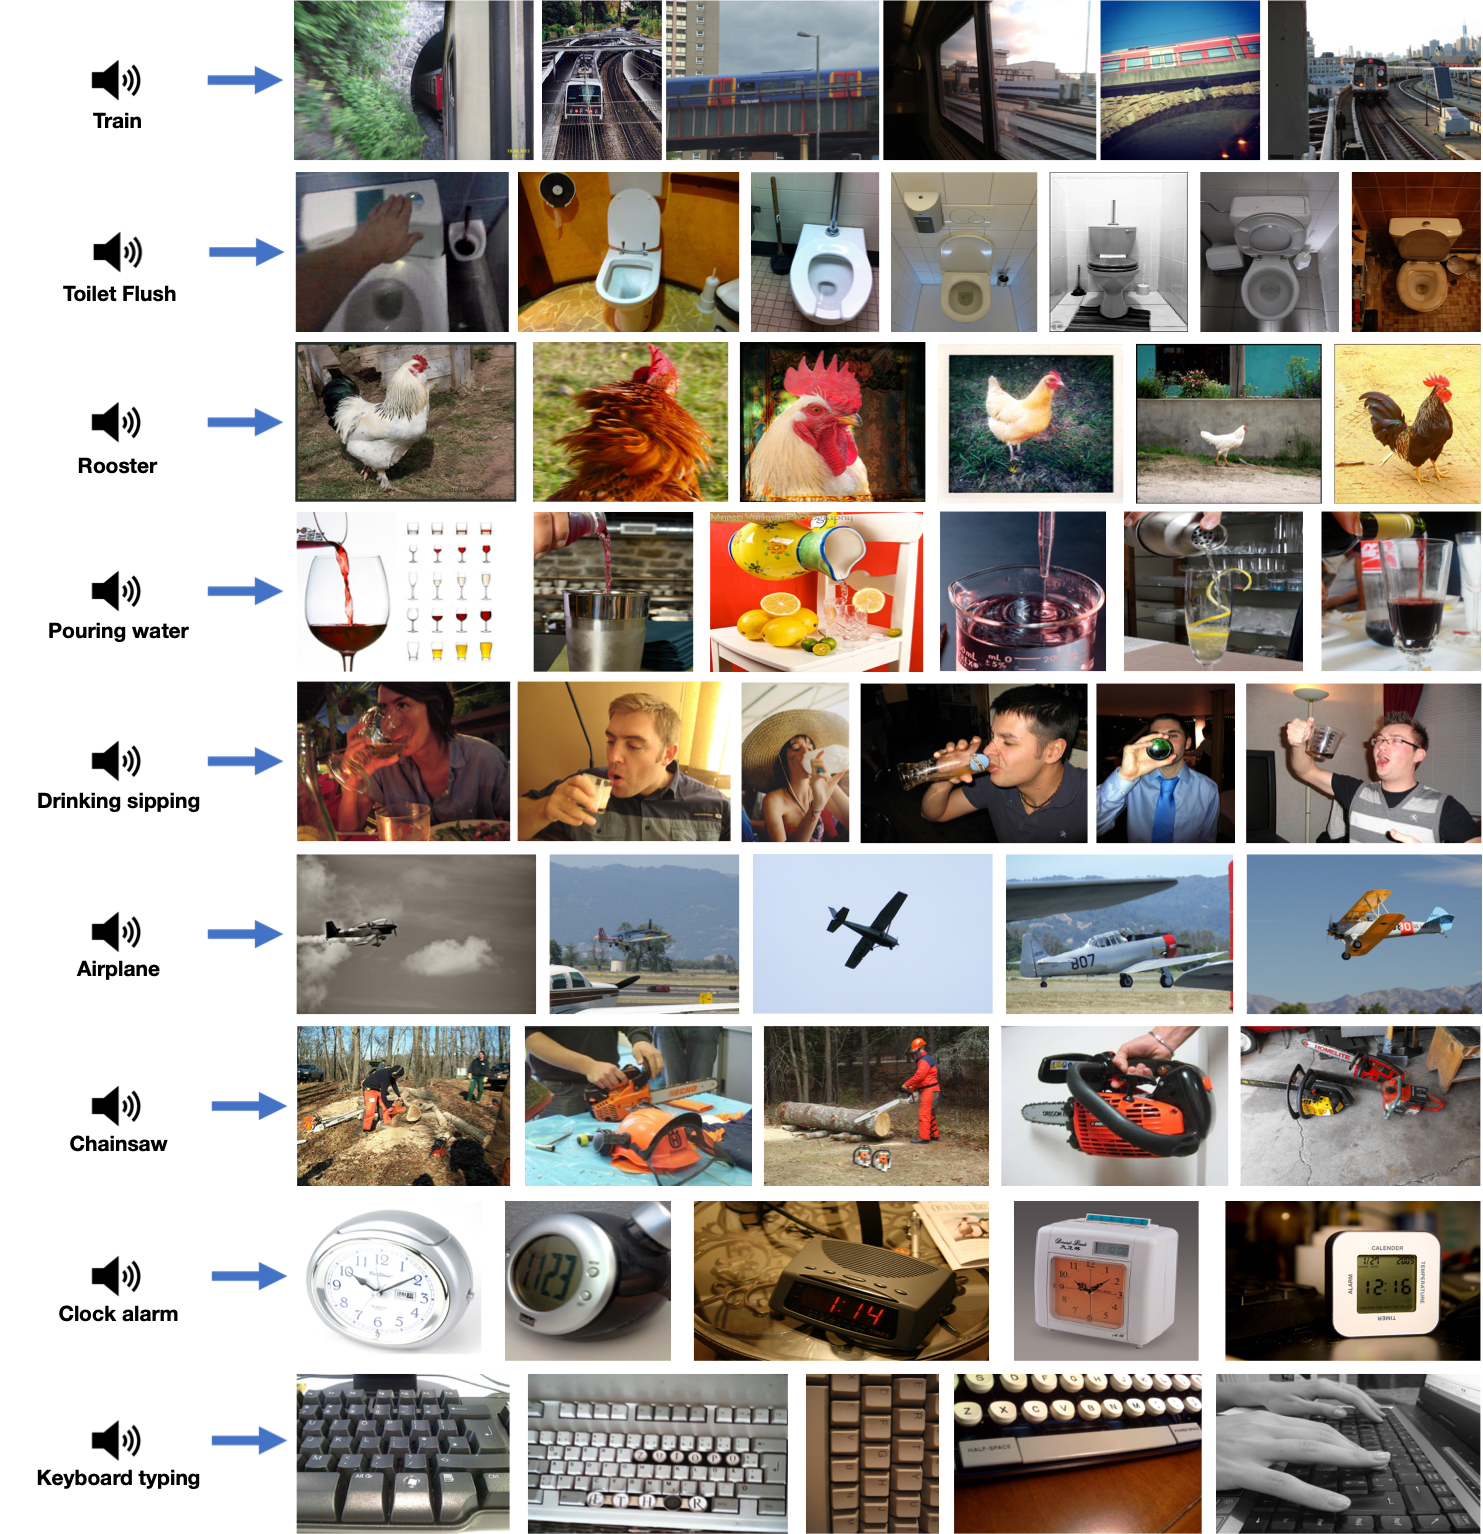
\includegraphics[width=\linewidth]{pic/audio2img_case_new.png}
    \caption{\textbf{Audio-to-image retrieval.}}
    \label{fig:audio2img}
\end{figure*}

\begin{figure*}[t]
    \centering
    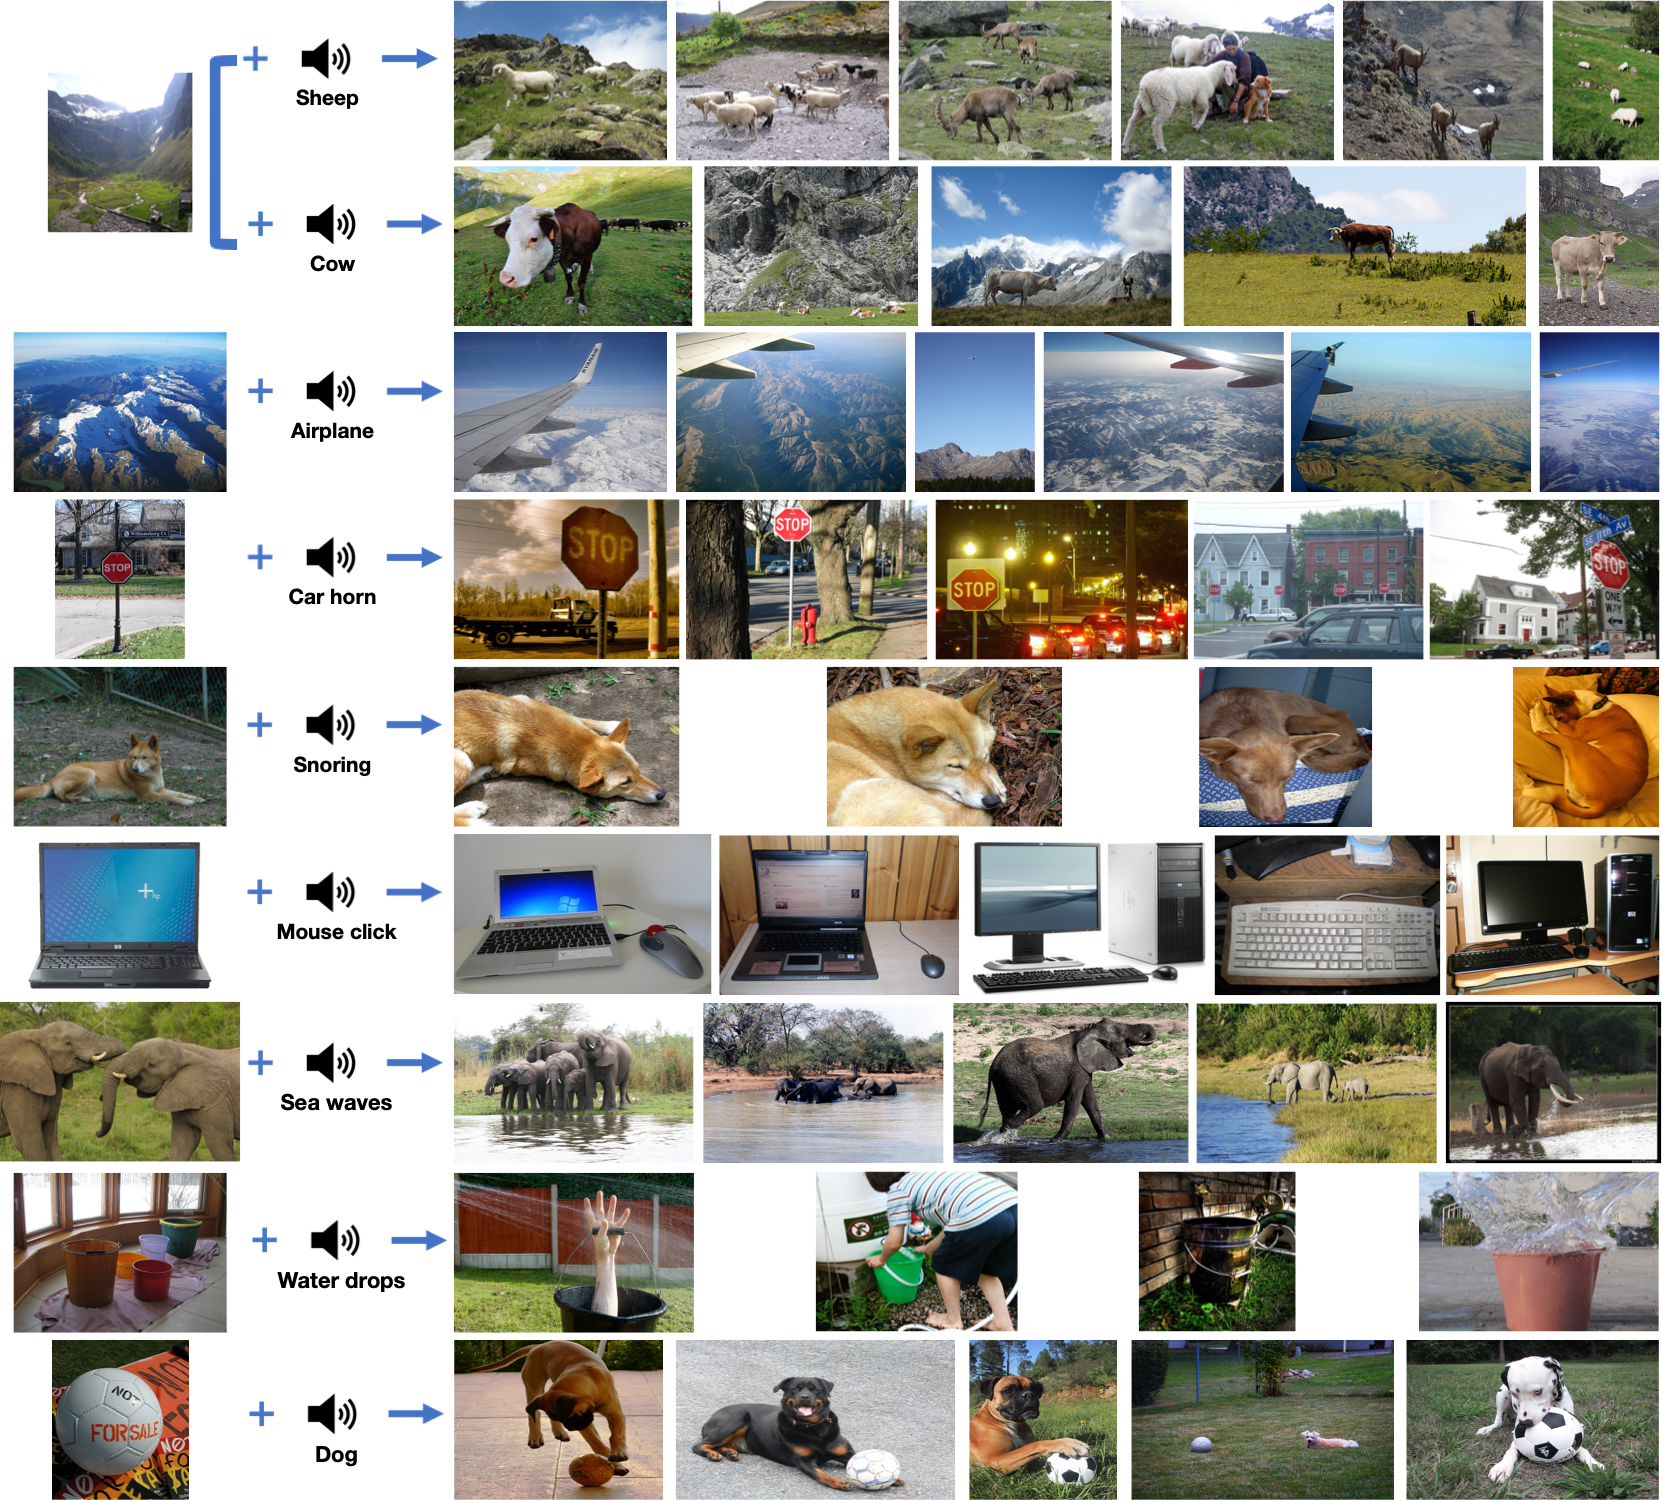
\includegraphics[width=\linewidth]{pic/audio+img2img_case_new.png}
    \caption{\textbf{Audio+image-to-image retrieval.}}
    \label{fig:audioimg2img}
\end{figure*}

\begin{figure*}[t]
    \centering
    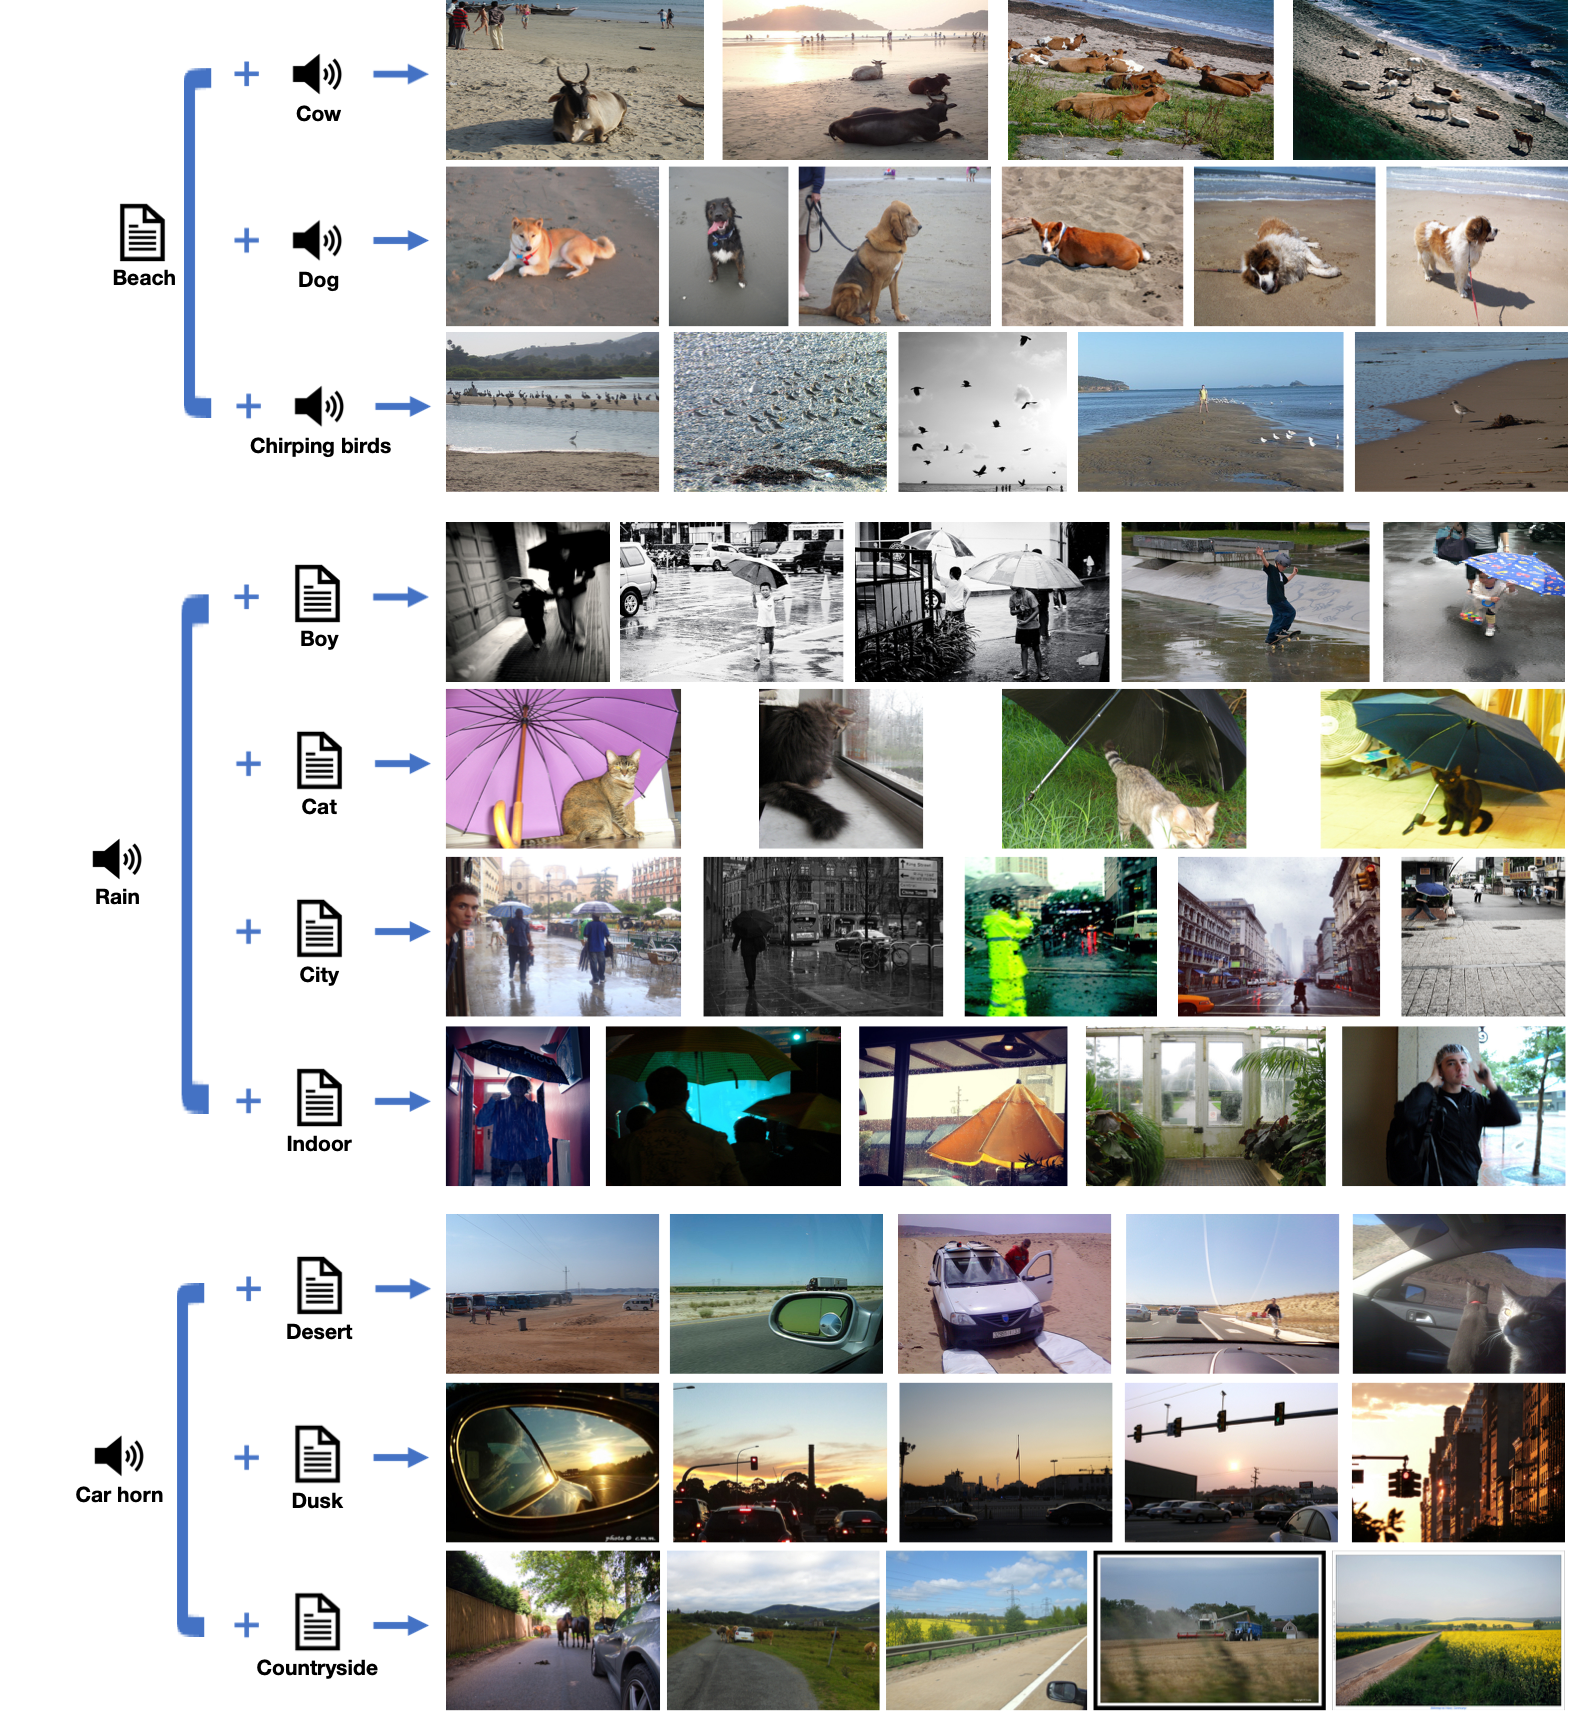
\includegraphics[width=\linewidth]{pic/audio+text2img_case_new.png}
    \caption{\textbf{Audio+text-to-image retrieval.}}
    \label{fig:audiotext2img}
\end{figure*}